\subsection{Extremwerprobleme}
\begin{LA}
	{Einführungsaufgabe}{}
	\begin{enumerate}


		\item Zwischen 08:00 Uhr und 18:00 Uhr wird in der Mensa der KS Im Lee die Lufttemperatur gemessen. Die Messungen wurden in das Koordinatensystem unten eingetragen. Wann ungefähr ist die Temperatur am höchsten? Wann am tiefsten?
		      \begin{center}
			      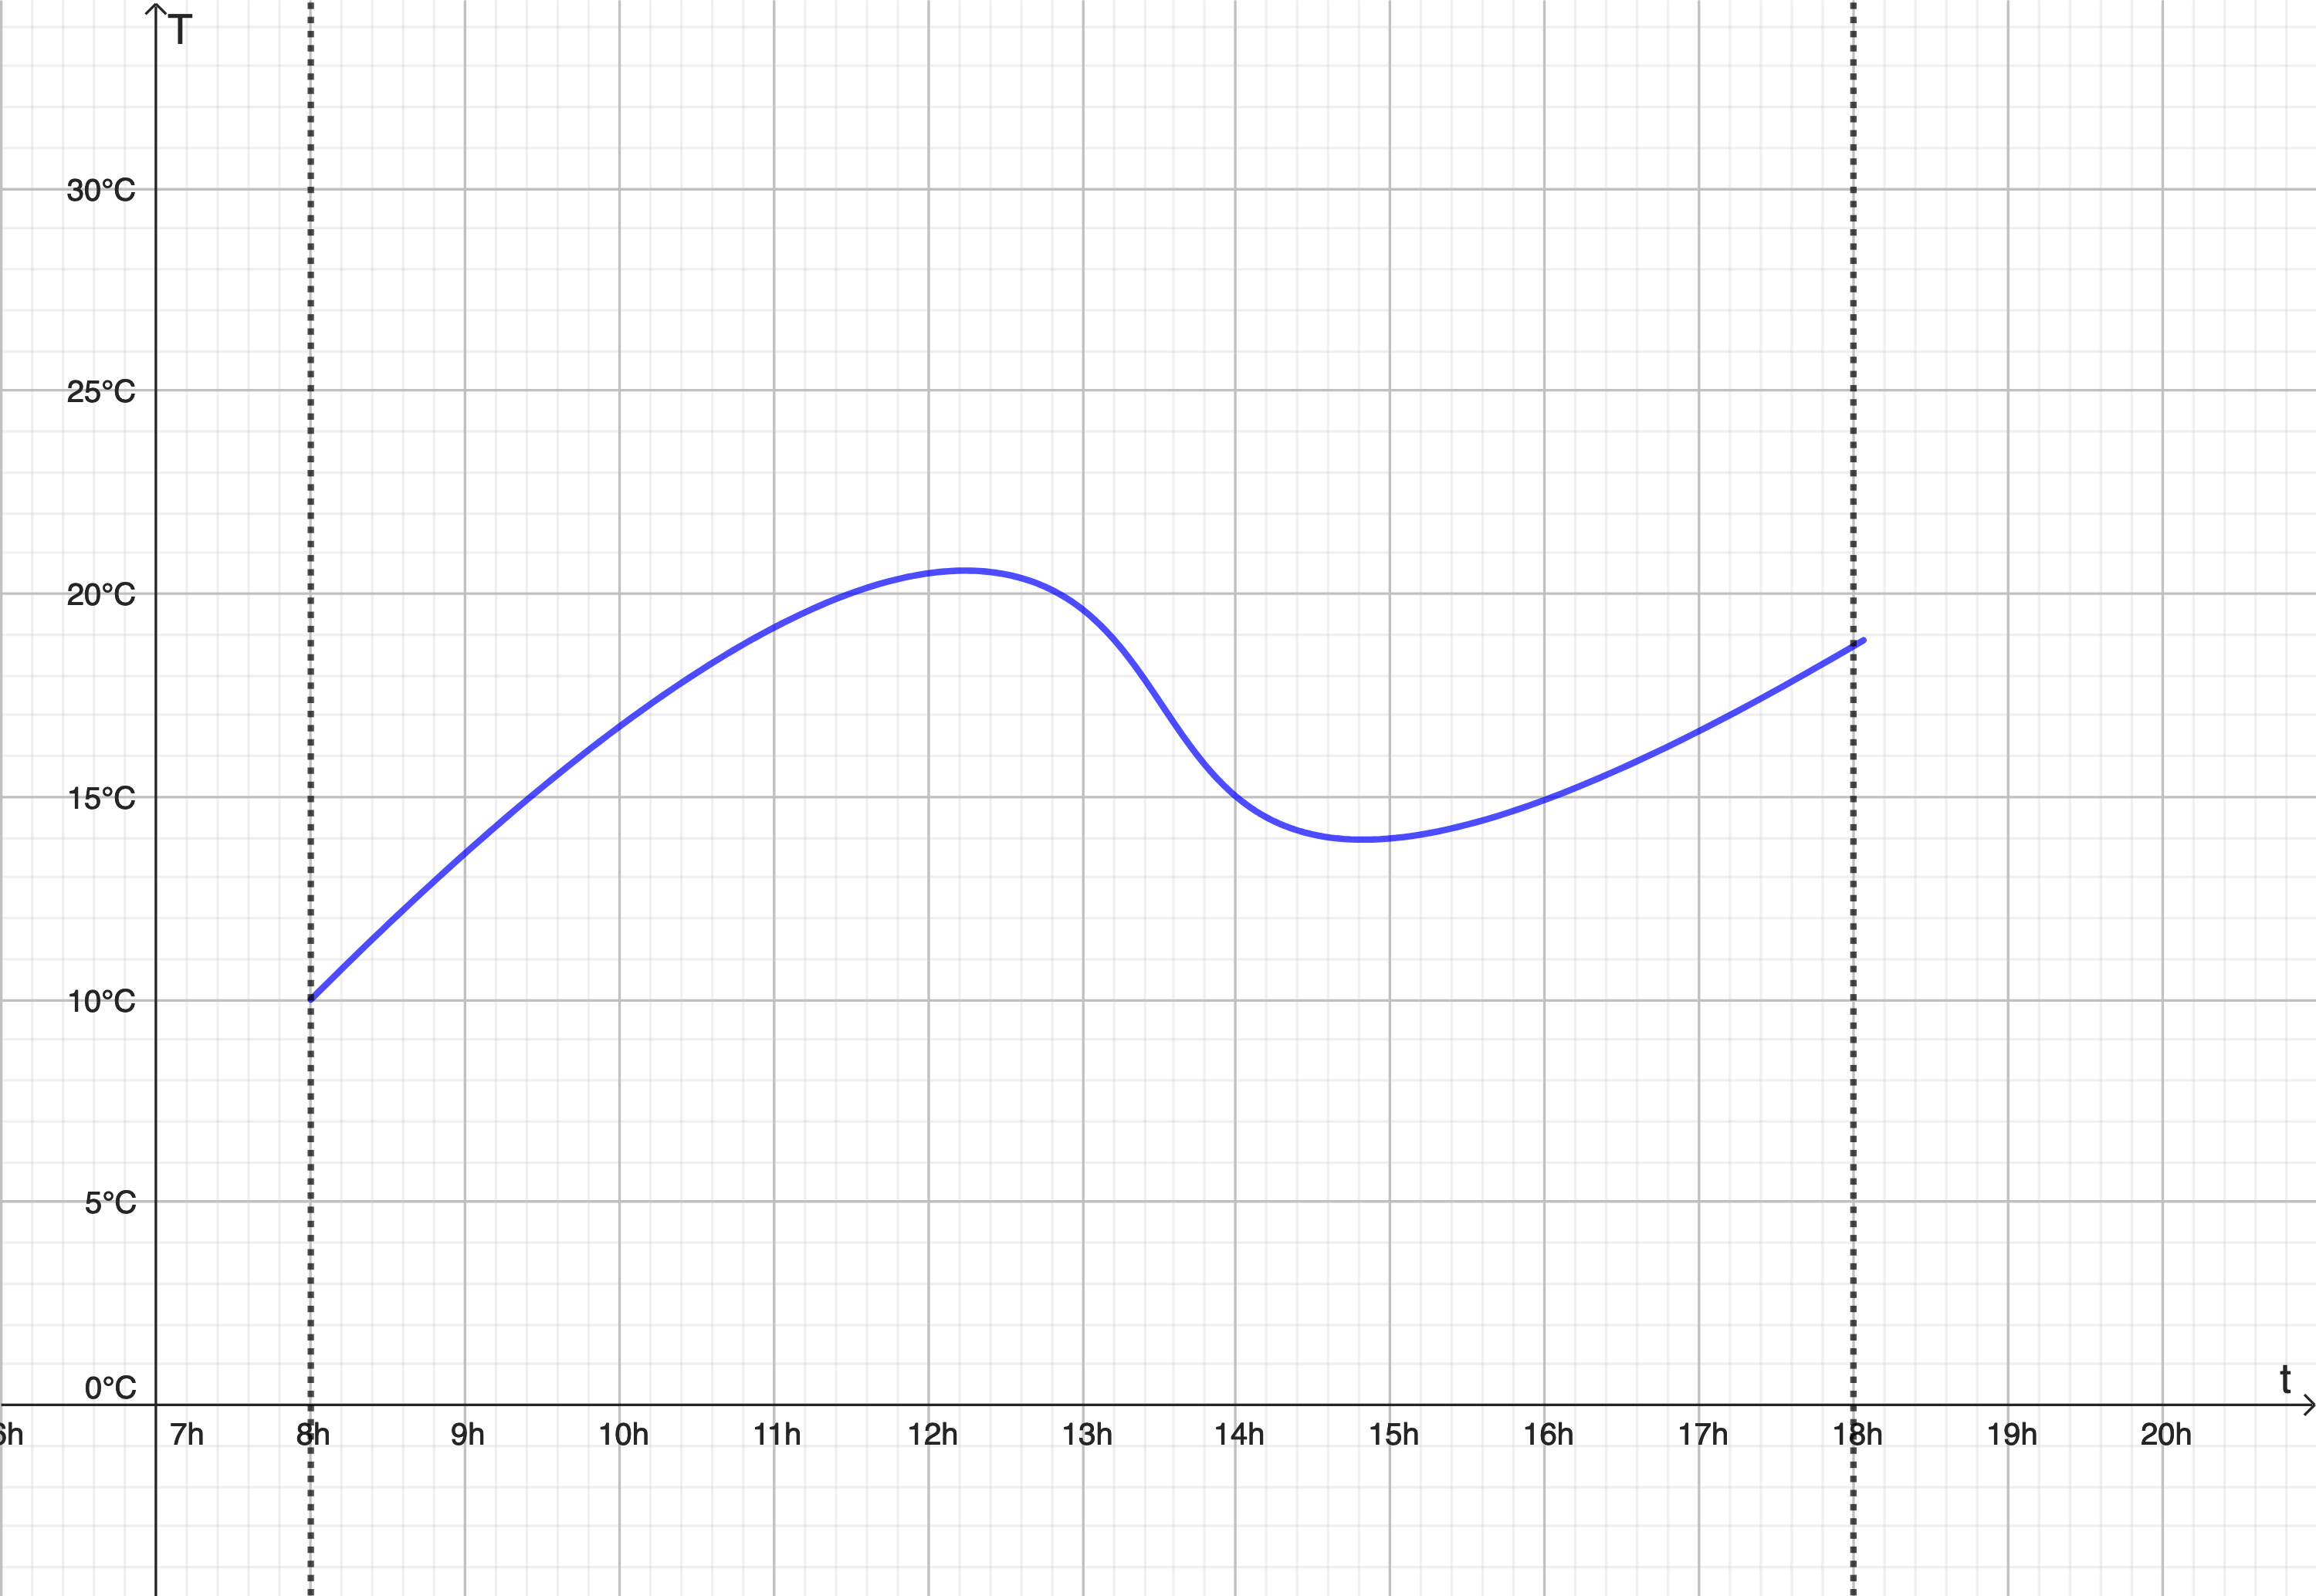
\includegraphics[width=0.9\textwidth]{media/globalMaxEaufgabe.png}
		      \end{center}

		\item Eine Flüssigkeit wird im Rahmen eines Experiments zuerst etwas aufgewärmt, dann in die Kälte gestellt. Der Temperaturverlauf während den ersten fünf Minuten des Experiments lässt sich durch die folgende Funktion modellieren: $T(t)=-t^2+4t+16$, für $t\in [0,5]$. Zu welchem Zeitpunkt in diesen ersten fünf Minuten war die Temperatur am höchsten? Wann am niedrigsten? (Es könnte hilfreich sein, den Graphen zu skizzieren).

		\item Bestimmen Sie den höchsten und niedrigsten Wert der Funktion $f(x)=x^3-3x$ im Intervall $x\in[-4, \frac{3}{2}]$.

		\item Gesucht ist der höchste Wert einer Funktion $f(x)$ im Intervall $x\in [a,b]$. Beschreiben Sie, wie man vorgehen soll, um die Aufgabe zu lösen. Welche Gleichungen muss man lösen? Welche Werte kommen infrage?
	\end{enumerate}

\end{LA}
\clearpage
\begin{definition}
	{Globale Extrema}{}
	Sei $f$ eine auf dem Intervall $[a,b]$ definierte, differenzierbare Funktion. Eine Stelle $x_0 \in [a,b]$ heisst \emph{globales Maximum} (bzw.\ \emph{Minimum}) der Funktion $f$ im Intervall $[a,b]$, falls für alle $x \in [a,b]$ gilt: $f(x) \le f(x_0)$ (bzw.\ $f(x)\ge f(x_0 )$).
\end{definition}

Betrachten Sie den folgenden Graphen einer Funktion im Intervall $[a,b]$

\begin{center}
	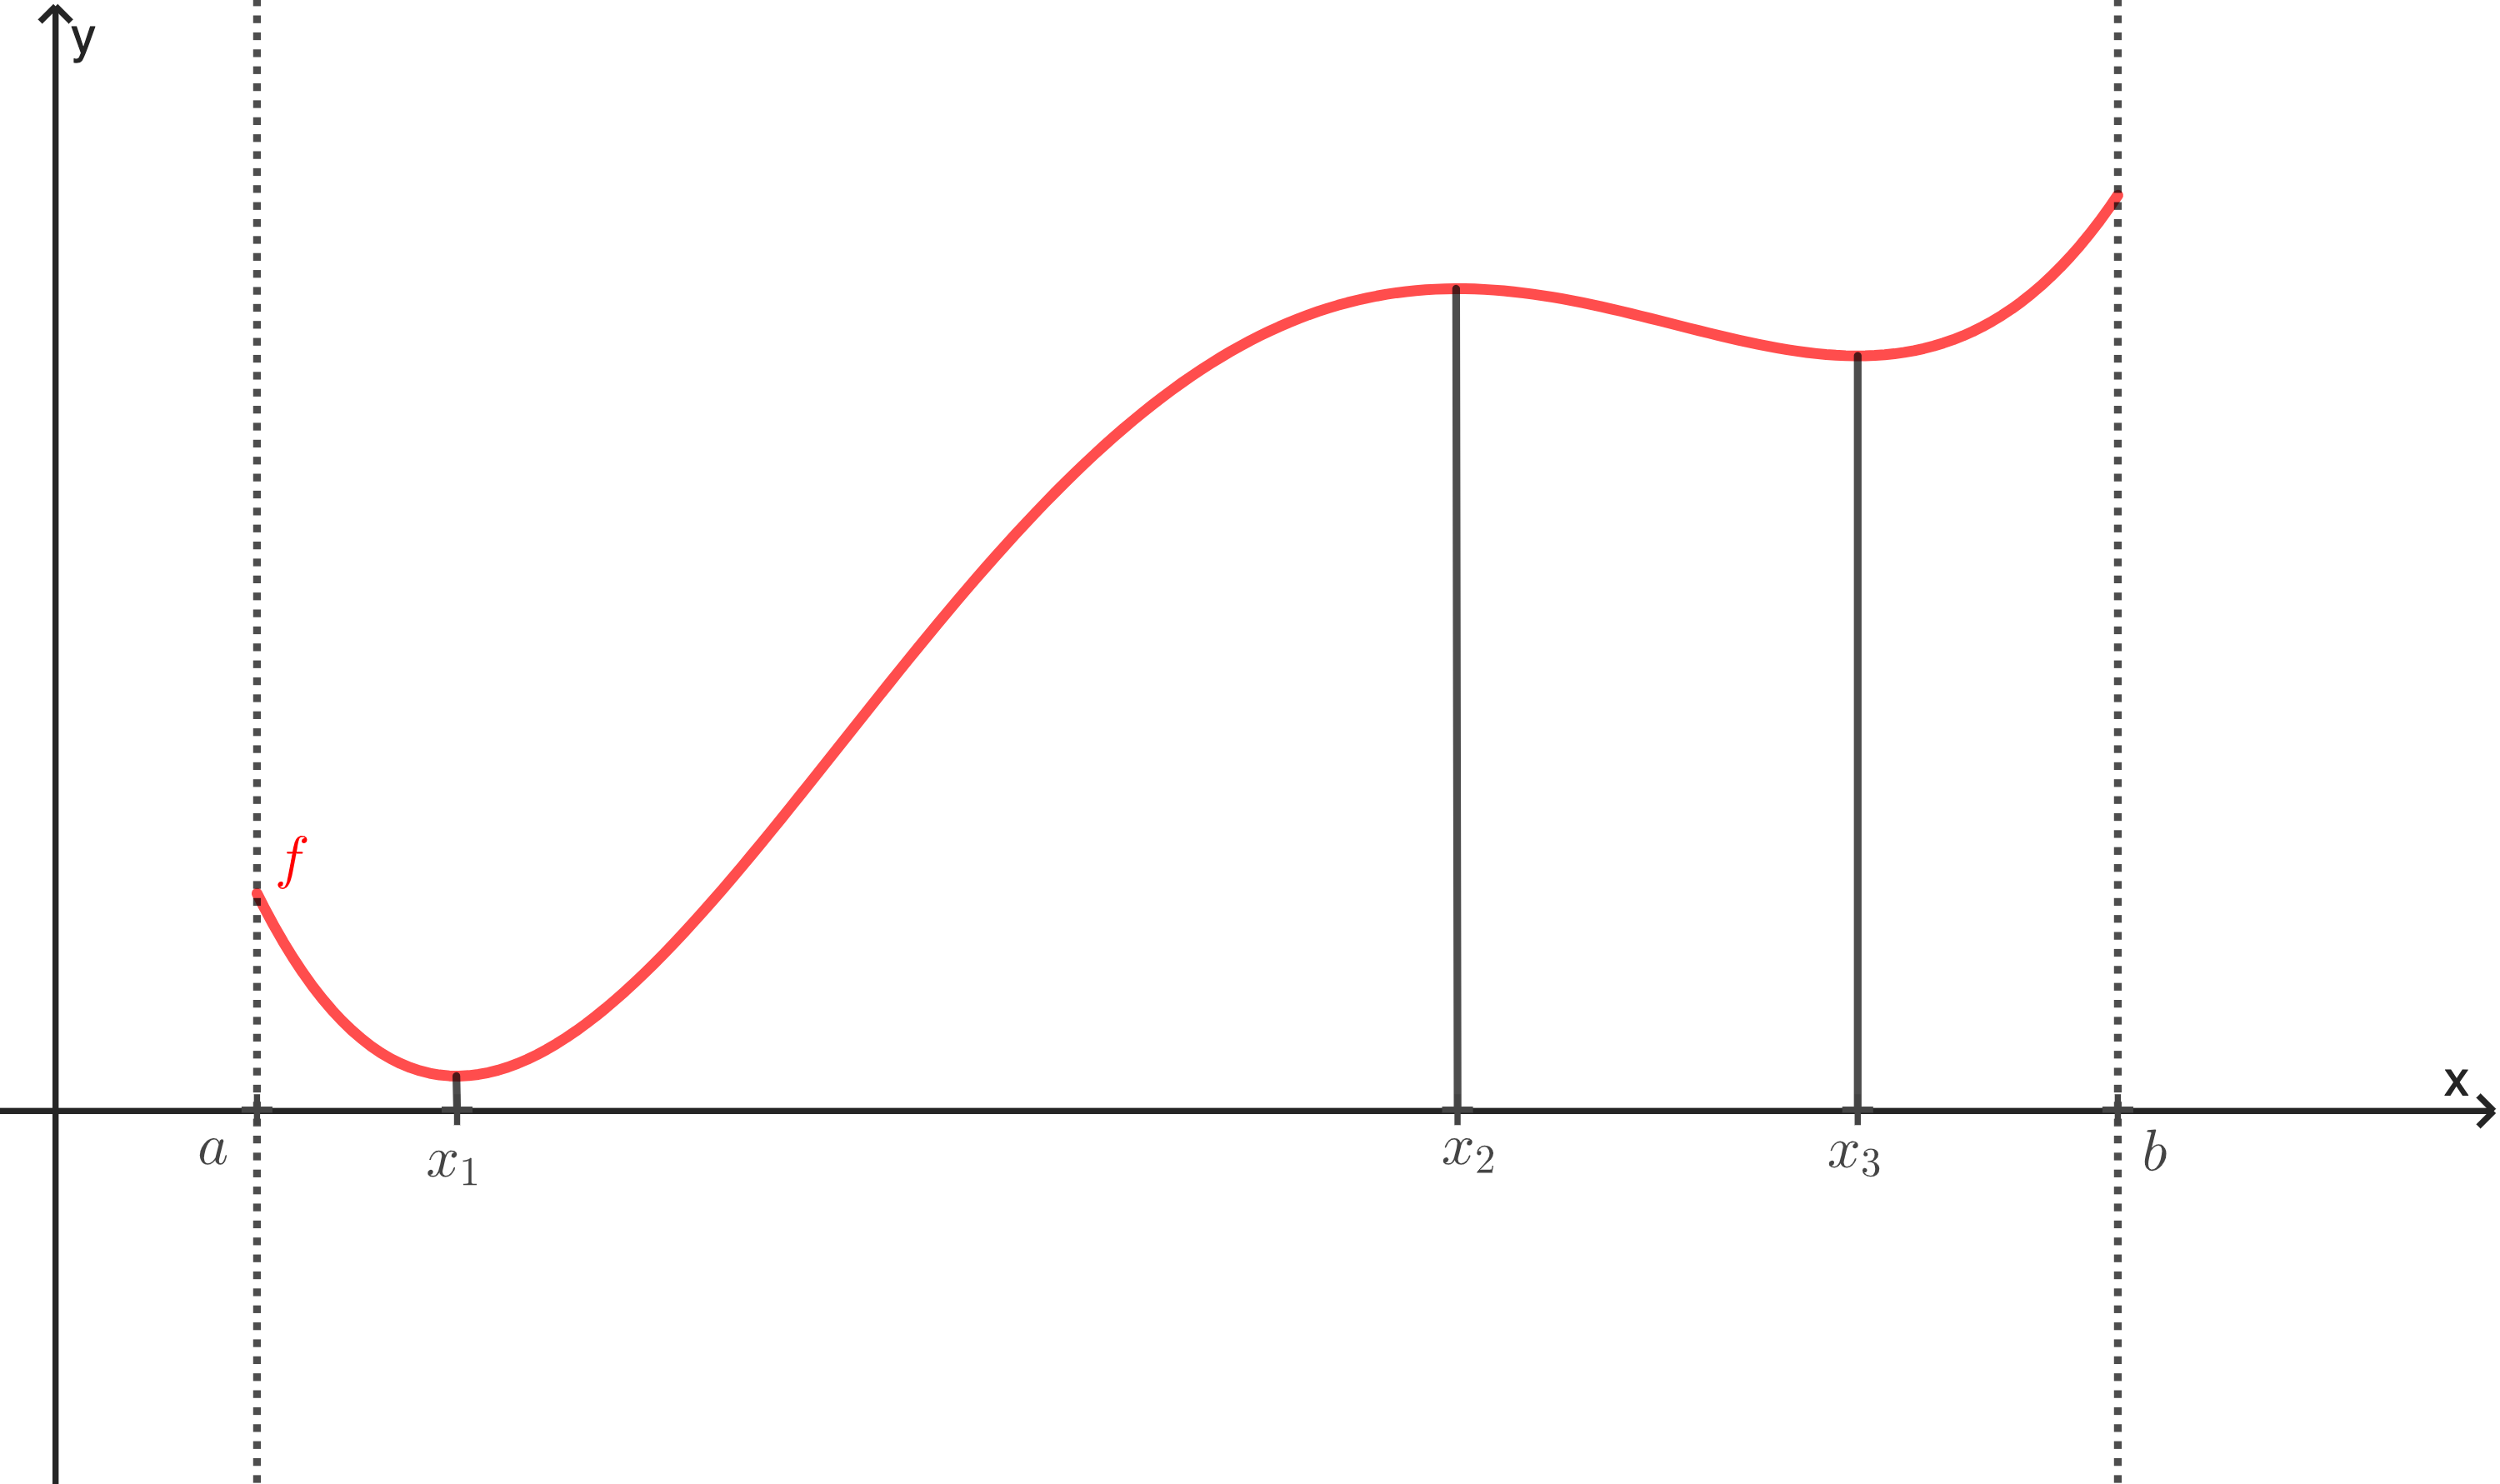
\includegraphics[width=0.6\textwidth]{media/globalExtremaDef.png}
\end{center}

Die Funktion hat die \textbf{lokalen} Extremalstellen $x_1,x_2$ und $x_3$.\\
Das \textbf{globale} Minimum ist an der Stelle $x_1$.\\
Das \textbf{globale} Maximum ist an der Stelle $b$.

Bei Anwendung sind oft die globalen Extremalstellen einer Funktion gesucht. Die Kosten wollen minimiert werden, der Ertrag will maximiert werden, usw.

Zum Auffinden der globalen Extremalstellen einer Funktion $f$ im Intervall $[a,b]$ kann man wie folgt vorgehen:
\begin{enumerate}
	\item Finde alle Stellen $x_1,x_2,\ldots ,x_n$ mit $f' (x)=0$ (Nullstellen der Ableitung).
	\item Die Kandidaten für das globale Extremum sind $x_1,x_2,\ldots ,x_n,a$ und $b$.
	\item Vergleiche die Werte $f(x_1 ),f(x_2 ),\ldots ,f(x_n ),f(a)$ und $f(b)$.
\end{enumerate}

\begin{bsp}
	{Globales Maximum der Funktion $f(x)=x^3-3x$ im Intervall $x\in [-4, \frac{3}{2}]$.}{}
	\begin{enumerate}
		\item $f'(x)=3x^2-3 \stackrel{!}{=} 0 \iff x_{1,2}=\pm 1$.
		\item Kandidaten: $x_1=-1,x_2=1,a=-4,b=\frac{3}{2}$.
		\item Vergleich:
		      \begin{center}
			      \begin{tabular}{c|| c|c|c|c}
				      $x$    & $-4$  & $- 1$ & $1$  & $\frac{3}{2}$ \\ \hline
				      $f(x)$ & $-52$ & $2$   & $-2$ & $-1.125$
			      \end{tabular}
		      \end{center}

		      Das globale Maximum im Intervall $x\in [-4,3/2]$ wird an der Stelle $x=-1$ erreicht, das globale Minimum an der Stelle $x=-4$.
	\end{enumerate}
\end{bsp}

\begin{bsp}
	{Musteraufgabe: Die beste Schachtel}{}
	Von einer A4-Seite ($21 \times 29$ cm) werden an den Ecken Quadrate mit der Seitenlänge $x$ cm abgeschnitten. Wie ist $x$ zu wählen, damit der Rest durch Falten eine Schachtel (ohne Deckel) mit maximalem Inhalt ergibt?

	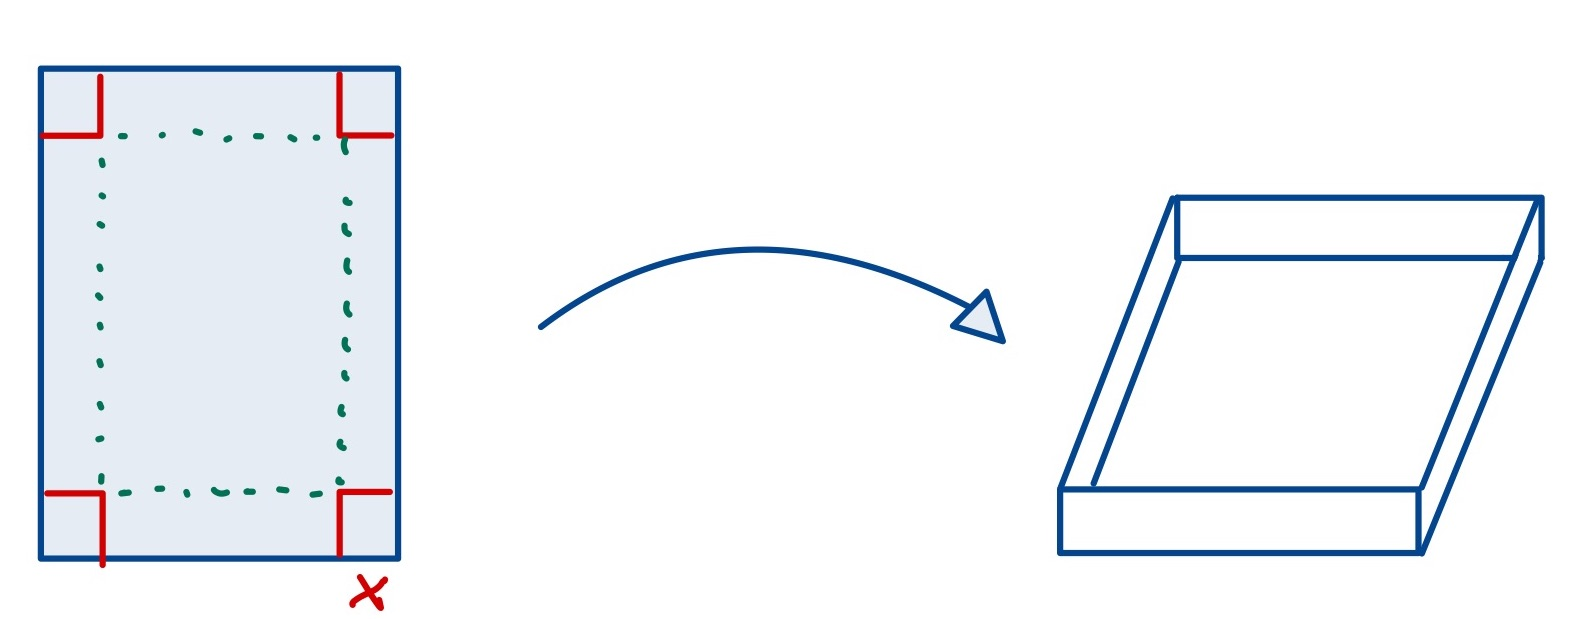
\includegraphics[width = 0.4\textwidth]{media/besteSchachtel.jpg}

	\vspace{14cm}
\end{bsp}

\pagebreak


\pagebreak
\begin{bsp}
	{Musteraufgabe: Ersatzfunktion}{Ersatzfunktion}
	Welcher Punkt der Parabel $y=x^2$ liegt am nächsten zum Punkt $A=(0,1)$?
	\vspace*{19cm}

	% \tcbvfill
\end{bsp}
\pagebreak
\begin{ueb}
	{Extremalprobleme}{}
	\begin{enumerate}
		\item Der Karton ist 40\,cm lang und 25\,cm breit. Es soll eine Schachtel mit Deckel entstehen. Wie lang sind die Kanten der Schachtel mit maximalem Inhalt?
		      \begin{center}
			      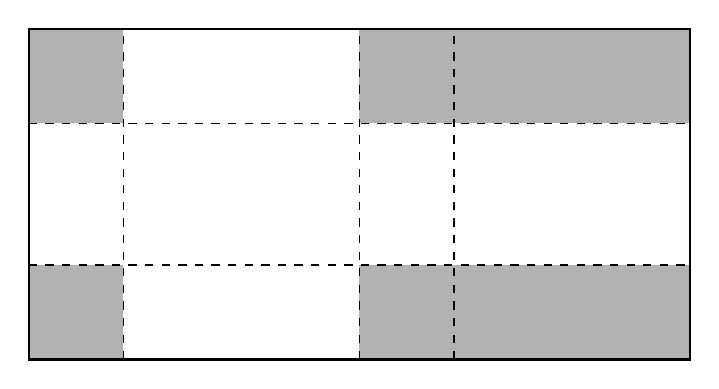
\begin{tikzpicture}[scale=0.12]
				      %% Dunkle Felder oben
				      \fill[gray!60] (0,20) rectangle (10,30);
				      \fill[gray!60] (35,20) rectangle (45,30);

				      %% Dunkle Felder unten
				      \fill[gray!60] (0,-5) rectangle (10,5);
				      \fill[gray!60] (35,-5) rectangle (45,5);

				      %% Dunkle Felder rechts (vertikale Doppelzone)
				      \fill[gray!60] (45,-5) rectangle (70,5);
				      \fill[gray!60] (45,20) rectangle (70,30);

				      %% Linienraster
				      \draw[thick] (0,-5) rectangle (70,30);
				      \draw[dashed] (10,-5) -- (10,30);
				      \draw[dashed] (35,-5) -- (35,30);
				      \draw[dashed]  (45,-5) -- (45,30);
				      \draw[dashed]  (0,5) -- (70,5);
				      \draw[dashed]  (0,20) -- (70,20);

			      \end{tikzpicture}
		      \end{center}
		\item Das Kantenmodell eines Quaders, der dreimal so lang wie breit ist, wird aus 520\,cm Draht hergestellt. Wie sind die Kanten zu wählen, wenn die Oberfläche des Quaders möglichst gross sein soll?
		      % \item Ein Kreissektor von gegebenem Umfang \(u\) soll maximalen Flächeninhalt haben. Bestimmen Sie den Radius und den Zentriwinkel des Sektors.
		\item Eine Blechbüchse soll so hergestellt werden, dass sie ein Volumen von 1 Liter hat. Wie sind die Abmessungen der Büchse zu wählen, damit sie möglichst wenig Material verbraucht?
		      % , wenn sie
		      %       \begin{enumerate}
		      % 	      \item einen Deckel und einen Boden hat?
		      % 	      \item keinen Deckel hat?
		      %       \end{enumerate}
		\item Wie hoch ist der gerade Kreiskegel mit gegebener Mantellinie \(s\), der grösstmögliches Volumen besitzt? Tipp: Sie können wählen, ob Sie die Höhe oder den Grundkreisradius als Variable verwenden wollen. Je nach Wahl der Variable kann die Zielfunktion einfacher oder kompliziert sein. Wählen Sie weise!
		\item Einem geraden Kreiskegel (Grundkreisradius \(3\,\text{cm}\), Höhe \(6\,\text{cm}\)) ist der Kreiszylinder mit maximalem Volumen einzubeschreiben, der die gleiche Rotationsachse wie der Kegel hat. Bestimmen Sie die Zylinderhöhe.
		      \newcounter{temp}
		      \setcounter{temp}{\value{enumi}}
	\end{enumerate}
\end{ueb}

\begin{ueb}
	{Noch mehr Extremalprobleme (nach \Cref{bsp:Ersatzfunktion})}{}
	\begin{enumerate}\setcounter{enumi}{\value{temp}}
		\item Welcher Punkt auf der Parabel \(p:\; y = 0.5x^{2}\) hat den kürzesten Abstand vom Punkt \(P(6, 0)\)? \\
		      Beim Lösen werden Sie vermutlich auf eine Gleichung dritten Grades stossen. Lösen Sie diese mit der Funktion poly-solv des Taschenrechners.
		\item
		      \begin{enumerate}
			      \item Skizzieren Sie die Parabel \(p:\; y = 5x - x^{2}\).
			      \item Der Punkt \(A(a, b)\) liegt im 1.\,Quadranten auf der Parabel \(p\). Bestimmen Sie die Koordinaten von \(A\) so, dass das Rechteck, von dem zwei Seiten auf den Koordinatenachsen liegen und von dem \(A\) eine Ecke ist, möglichst grossen Umfang hat.
		      \end{enumerate}
		\item Lösen Sie das gleiche Problem für die Parabel \(p:\; y = 3x - x^{2}\); diesmal soll das Rechteck maximalen Flächeninhalt haben.

		\item Die Parabel mit der Gleichung $y=\frac{1}{4}x^4+4$ und die zur $y$-Achse parallele Gerade an der Stelle $x=8$ begrenzen im 1. Quadranten ein Gebiet, in welches ein Rechteck mit grösstmöglichem Inhalt einbeschrieben werden soll. Die Seiten des Rechtecks sollen parallel zu den Koordinatenachsen verlaufen. Bestimmen Sie die Koordinaten der Ecke $P$ auf dem Parabelbogen.


		\item Dem Flächenstück, das die Parabel \(p:\; y = a - x^{2}\) \((a > 0)\) mit der \(x\)-Achse einschliesst, ist ein Rechteck so einzubeschreiben, dass es bei Rotation
		      \begin{enumerate}
			      \item um die \(y\)-Achse den Zylinder mit maximalem Volumen erzeugt;
			      \item um die \(x\)-Achse den Zylinder mit maximalem Volumen erzeugt. \\
			            Beim Lösen werden Sie vermutlich auf eine biquadratische Gleichung stossen. Lösen Sie diese mit einer Substitution der Form $t= u^2$ (Variablennamen entsprechend anpassen).
		      \end{enumerate}
		      Berechnen Sie die Seitenlängen dieses Rechtecks.
	\end{enumerate}


\end{ueb}

\pagebreak
\emph{Lösungen:}

\begin{enumerate}
	\item \(x = 5\,\text{cm}\), Schachtel: \(15 \times 15 \times 5\).
	\item Breite \(= 20\,\text{cm}\), Länge \(= 60\,\text{cm}\), Höhe \(= 50\,\text{cm}\).
	\item \(r = \sqrt[3]{\tfrac{1}{2\pi}} \text{ dm},\; h = 2r\).
	      %   \begin{enumerate}
	      %       \item \(r = \sqrt[3]{\tfrac{1}{2\pi}} \text{ dm},\; h = 2r\).
	      %       \item \(r = \sqrt[3]{\tfrac{1}{\pi}} \text{ dm},\; h = r\).
	      %   \end{enumerate}
	\item \(h = \tfrac{\sqrt{3}}{3}\,s\).
	\item \(h = 2\,\text{cm}\).
	\item \(x = 2,\; \text{Punkt} = (2,2)\).
	\item
	      \begin{enumerate}
		      \item %% nur Skizze, keine Kurzloesung noetig
		      \item \(A = \left(3,\, 6\right)\).
	      \end{enumerate}
	\item \(A = \left(2, 2\right)\).
	\item Es gibt zwei Lösungen: $P_1 = (0, 4); P_2=(4, 8)$. (Randextremum!)
	\item
	      \begin{enumerate}
		      \item \(2\sqrt{\frac{a}{2}}\text{ und } \frac{a}{2}\).
		      \item \(2\sqrt{\frac{a}{5}}\text{ und } \frac{4a}{5}\).
	      \end{enumerate}
\end{enumerate}

































\pagebreak

Anwendungsprobleme mit \glqq weiteren Funktionstypen\grqq{}:
\begin{bsp}
	{Das Baywatch-Problem}{}
	Ein Schwimmer gerät in Notlage. An welcher Stelle muss der Rettungsschwimmer Mitch ins Meer springen, damit er möglichst schnell bei der hilfsbedürftigen Person ankommt? Gehen Sie von folgenden Daten aus: An Land rennt Mitch mit einer Geschwindigkeit von 5 m/s. Seine Schwimmgeschwindigkeit beträgt 3 m/s. Die restlichen Masse entnehmen Sie der Skizze:
	\begin{center}
		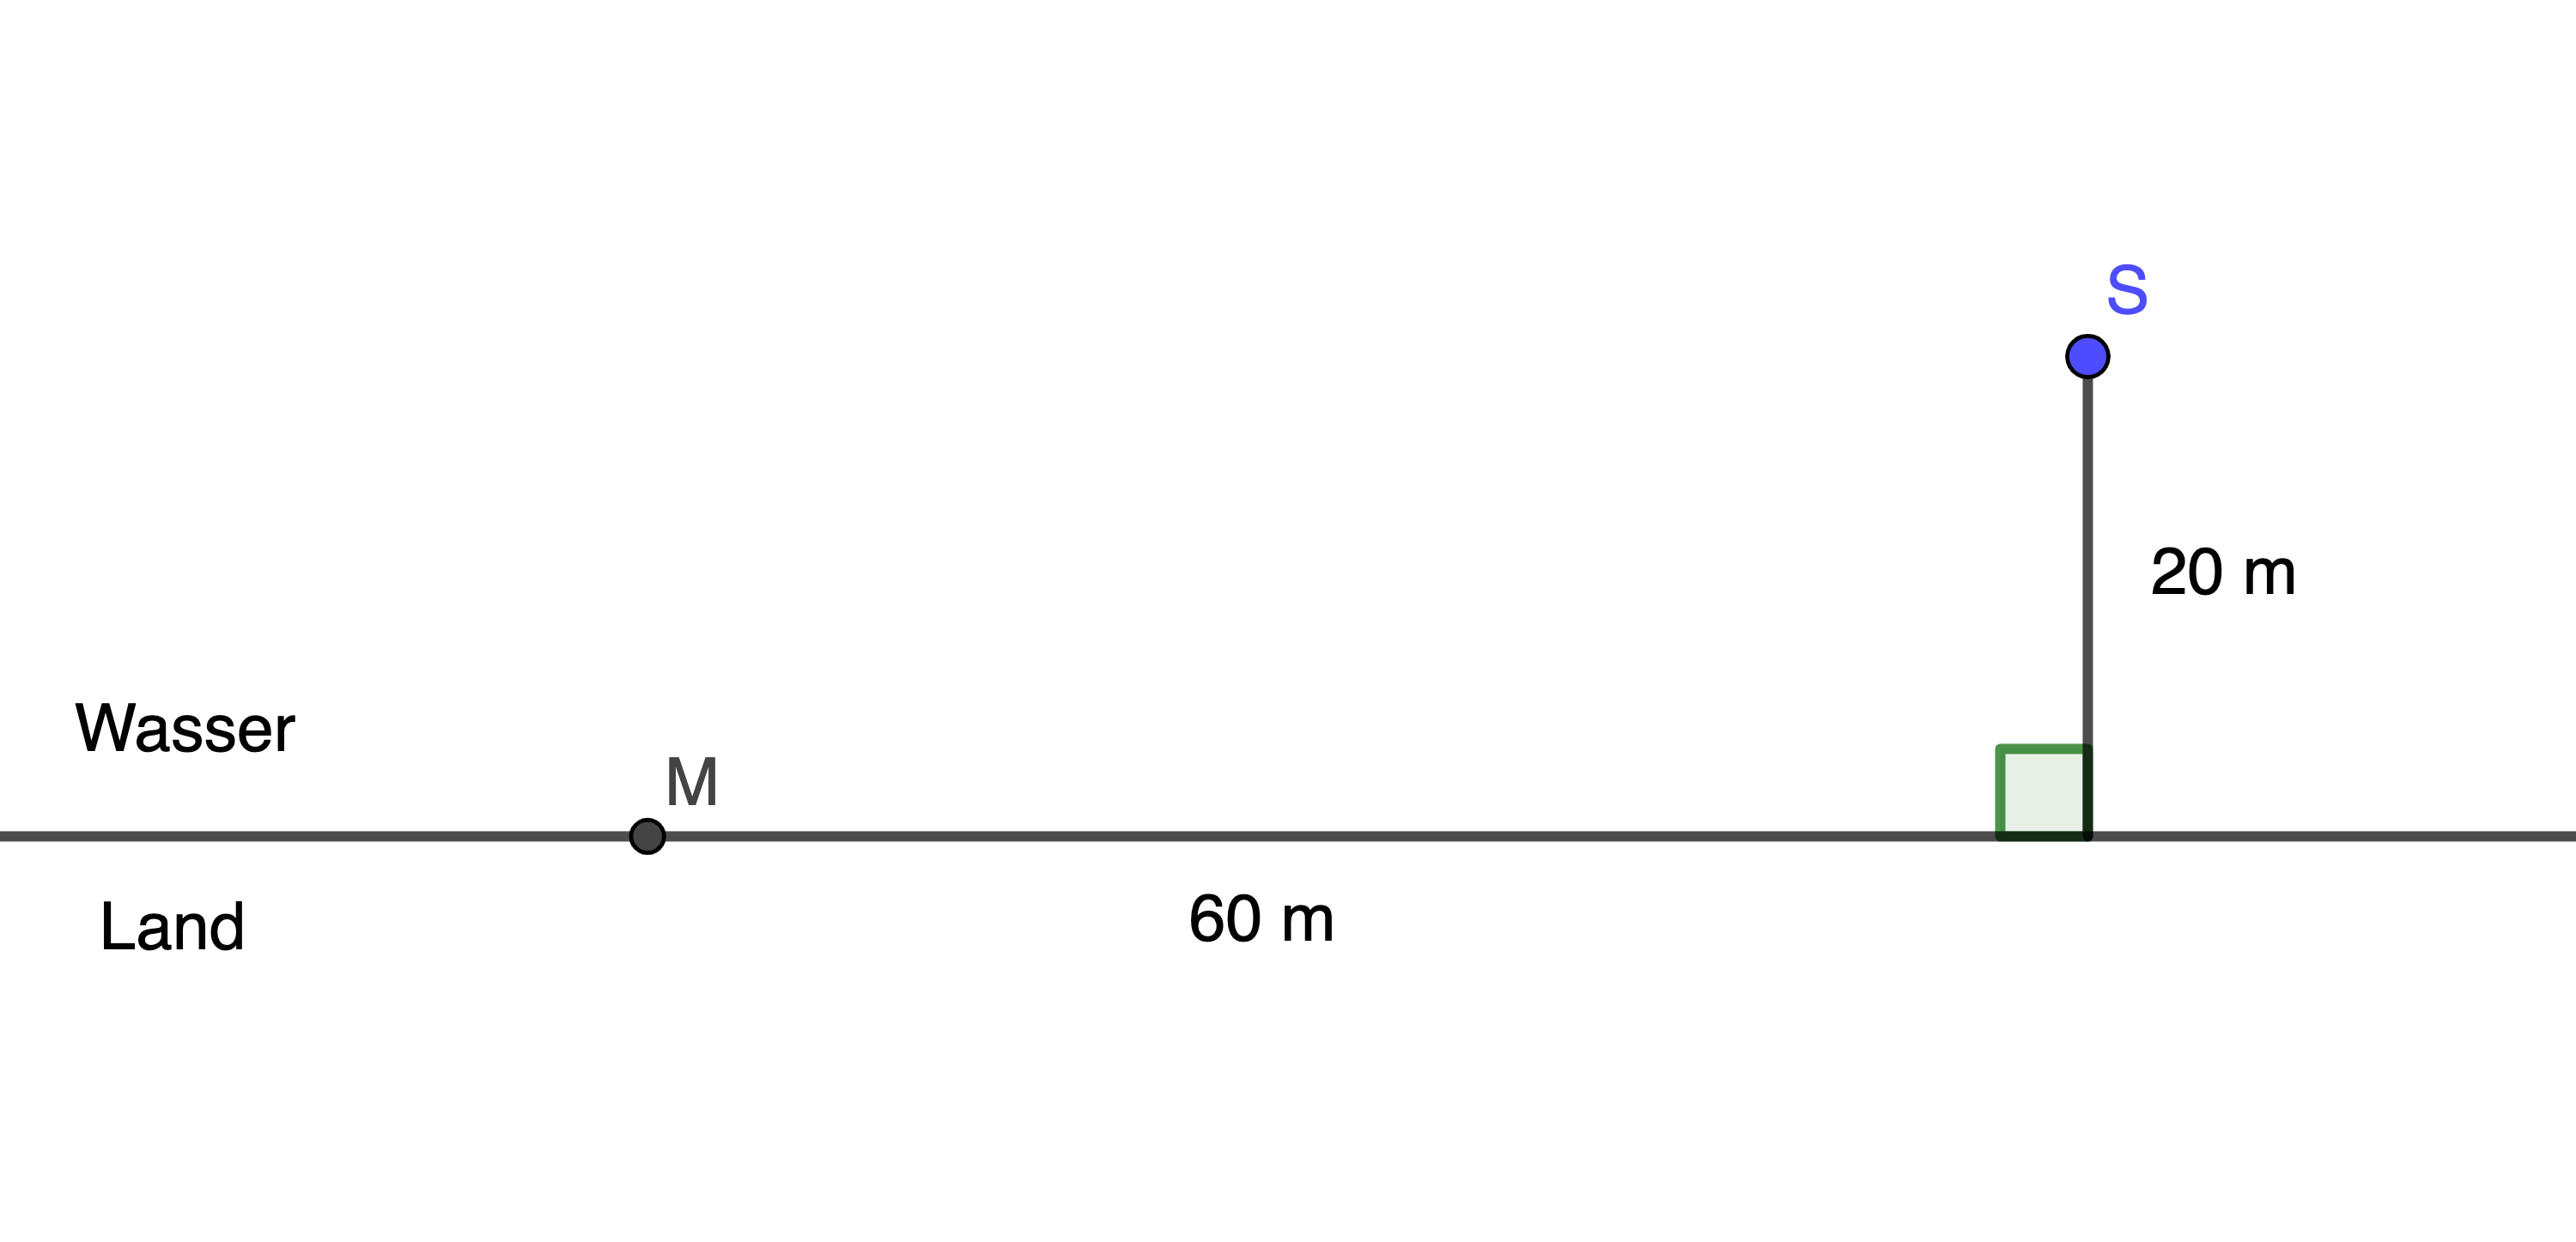
\includegraphics[width = 0.8 \textwidth]{media/baywatch.png}
	\end{center}
	\vspace*{10cm}
	\pagebreak
	\phantom{hallo}
	\vspace*{19cm}

\end{bsp}

\clearpage

\begin{bsp}
	{Bus optimal erwischen}{}
	Sie wohnen in der Entfernung 100 m von einer geraden Strasse. Jeden Morgen um 7Uhr fährt ein Bus mit der Geschwindigkeit 4 m/s vorbei, auf den Sie mit 2 m/s rennend jeweils aufspringen. In welchem Winkel $x$ zum Lot der Strasse müssen Sie jeweils losrennen, damit Sie möglichst spät von zu Hause wegrennen können?

	\vspace*{18 cm}

\end{bsp}

\clearpage

\begin{ueb}
	{}{}
	\begin{enumerate}
		\item Was vermuten Sie: Welches von allen gleichschenkligen Dreiecken mit dem Umfang 24\,cm hat den grössten Flächeninhalt? Beweisen Sie Ihre Vermutung, indem Sie das entsprechende Extremalproblem lösen. Hinweis: Sie können die Zielfunktion mit Produkt- und Kettenregel ableiten, oder Sie formen sie so um, dass Sie eine Ersatzfunktion verwenden können. Beides geht.
		\item Einem Rechteck wird ein gleichschenkliges Dreieck aufgesetzt (siehe Skizze). Wie breit muss das Rechteck sein, damit der Flächeninhalt der ganzen Figur maximal wird? Hinweis: Hier werden Sie vermutlich die Produkt- und die Kettenregel verwenden müssen. Vergessen Sie bei der Wurzelgleichung die Probe nicht.
		      \begin{center}
			      %% TikZ-Code fuer die dargestellte Figur

			      \begin{tikzpicture}[scale=2]
				      %% Untere Basis
				      \draw (0,0) -- (3,0);

				      %% Seitenwaende (Hoehe 1)
				      \draw (0,0) -- (0,1);
				      \draw (3,0) -- (3,1);

				      %% Schraegdaecher mit Laenge 2
				      %% %% Hinweis: Exakte Position des Firstpunkts im Bild unklar
				      %% %% daher angenommene symmetrische Position
				      \draw (0,1) -- (1.5,2);
				      \draw (3,1) -- (1.5,2);

				      %% Beschriftungen
				      \node[left] at (0,0.5) {1};
				      \node[right] at (3,0.5) {1};
				      \node[above] at (0.75,1.5) {2};
				      \node[above] at (2.25,1.5) {2};
			      \end{tikzpicture}

		      \end{center}



		\item $$f(x) = e^{-x^2}$$
		      \begin{enumerate}
			      \item Der Ursprung des Koordinatensystems ist die Spitze eines gleichschenkligen Dreiecks; die Endpunkte der Basis liegen auf dem Graphen von \(f\). Das Dreieck soll maximalen Flächeninhalt haben. Welche Koordinaten haben die Endpunkte der Basis?
			      \item Zeigen Sie, dass die in a. gefundenen Punkte den Wendepunkten der Funktion \(f\) entsprechen.
		      \end{enumerate}


		\item Die Punkte \(A(3,3)\) und \(B(0,2)\) sind gegeben. Der Punkt \(C\) liegt auf der Kurve \(f\colon y=\ln x\). Das Dreieck \(ABC\) soll minimalen Flächeninhalt haben. Welche Koordinaten hat \(C\)? Tipp: Hier empfiehlt sich ein ganz anderer Lösungsweg. Was kann man über die Kurventangente in $C$ sagen?

	\end{enumerate}

\end{ueb}

\clearpage
%% Kurzloesungen

\begin{enumerate}
	\item Seiten \(8,8,8\) (Gleichseitiges Dreieck).

	\item Rechteckbreite \(=2\sqrt{3}\).



	\item
	      \begin{enumerate}
		      \item Endpunkte \( P_{1,2} = (\pm \tfrac{1}{\sqrt{2}},\, e^{-1/2}) \).
		      \item Rechne nach: $f''(\pm \tfrac{1}{\sqrt{2}}) = 0$ und $f'''(\pm \tfrac{1}{\sqrt{2}}) \neq 0$.
	      \end{enumerate}
	\item Minimaler Flaecheninhalt des Dreiecks \(ABC\): Punkt \(C=(3,\ln(3))\).
\end{enumerate}

\clearpage

\begin{ueb}
	{Optimale Geschwindigkeit einer Autokolonne}{}
	% Zu hohes Verkehrsaufkommen auf einer engen Strasse \dots wieder ein Stau! Je grösser das Verkehrsaufkommen, desto langsamer bewegt sich die Autokolonne. Bei kleinen Geschwindigkeiten können mehr Autos passieren.

	% Diese Feststellung ist insofern etwas eigenartig, als bei 0 km/h überhaupt kein Auto fährt. Gibt es eine optimale Geschwindigkeit für eine Autokolonne?

	Wichtig bei Autokolonnen ist der Sicherheitsabstand zwischen Fahrzeugen. Je grösser die Geschwindigkeit der Kolonne, desto grösser muss der Abstand sein und das hat einen Einfluss auf den Durchfluss. Umgekehrt ist der Abstand bei kleinen Geschwindigkeiten klein, aber im Schneckentempo ist der Durchfluss auch nicht gerade gross.
	Eine Faustregel der Polizei sagt:
	\[r\approx0.0075 v^2 \quad \text{$v$ in km/h, $r=$ Bremsweg in m}\]

	\begin{enumerate}
		\item Wie viele Meter Abstand zum vorderen Fahrzeug müsste eine Automobilistin bei einer Geschwindigkeit von 60 km/h mindestens einhalten?
		\item Stellen Sie sich vor, eine Kolonne habe eine Geschwindigkeit von 60 km/h und bestehe aus lauter Personenwagen. Der Einfachheit halber nehmen wir an, dass jedes Auto eine Länge von 4 m habe und dass alle Automobilistinnen und Automobilisten den vorgeschriebenen Abstand einhalten.
		      An einer gewissen Stelle hat die Polizei eine Zählstation aufgestellt.
		      \begin{center}
			      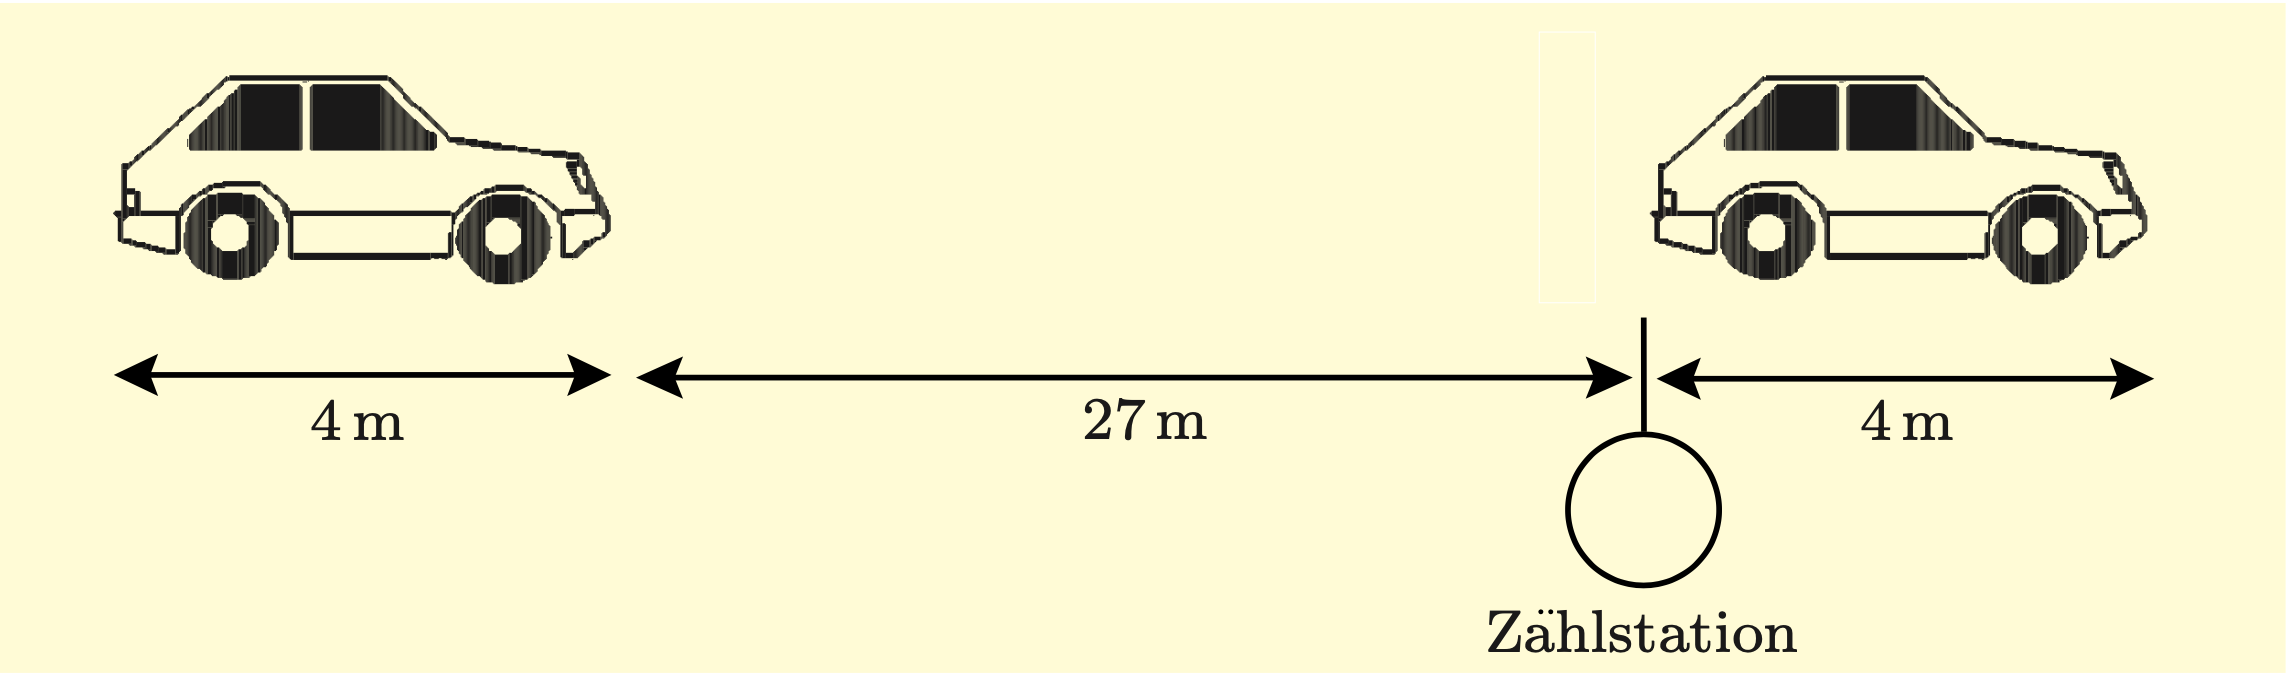
\includegraphics[width = 0.8 \textwidth]{media/auto-zaehlstation-neu.png}
		      \end{center}
		      Zeigen Sie, dass pro Minute ungefähr 32 Autos vorbeifahren können.
		\item Wie viele Autos können bei einer Geschwindigkeit von 120 km/h bei der Zählstation vorbeifahren?
		\item Die Anzahl Autos $N$, welche die Zählstation pro Minute passieren können, ist eine Funktion der Geschwindigkeit $v$ in km/h.
		      \\ Zeigen Sie, dass gilt
		      \[ N(v)=\frac{1000v}{0.45v^2+240}\]
		\item Zeichnen Sie den Graphen der Funktion mit Geogebra und kontrollieren Sie, dass der maximale Durchfluss einer Kolonne unter den oben skizzierten Bedingungen bei ungefähr 25 km/h liegt.
		\item Berechnen Sie $\frac{dN}{dv}$ und benutzen Sie das Resultat, um die optimale Geschwindigkeit auszurechnen.
		\item Wie beurteilen Sie das Modell? Machen Sie Vorschläge für Verbesserungen und Untersuchen Sie die daraus resultierende optimale Geschwindigkeit.

	\end{enumerate}

\end{ueb}
